\section{Model}

A story is represented by a series of states $s_i$ and actions $a_j$.
Each story starts in some initial state $s_0$, then one or more actions happen
($a_0, ..., a_j$), which lead to $s_1$. This pattern continues until the final 
state of the story, which is where the story ends.

The story sequence is assumed to have some temporal relations too. To represent
events happening in parallel, stories can contain stories themselves too.
\begin{figure}
	\begin{tikzpicture}[remember picture,
		outer/.style={draw=green,fill=green!20,thick,inner sep=10pt}
	]
		\node[outer,draw=green] (s1) at (0,0) {
			\begin{tikzpicture}
				\node[shape=rectangle,draw=black] (1p) at (0,0) {princess};
				\node[shape=rectangle,draw=black] (1pac) at (3.5,2) {princess\_abilities:companionship};
				\node[shape=rectangle,draw=black] (1pnb) at (3.5,-2) {princess\_needs:ball};
				\node[shape=rectangle,draw=black] (1pr1) at (7,0.75) {promise:1};
				\node[shape=rectangle,draw=black] (1pr2) at (7,-0.75) {promise:2};
				\node[shape=rectangle,draw=black] (1fab) at (10.5,2) {frog\_abilities:ball};
				\node[shape=rectangle,draw=black] (1fnc) at (10.5,-2) {frog\_needs:companionship};
				\node[shape=rectangle,draw=black] (1f) at (15,0) {frog};

				\draw[-] (1p) -- (1pac);
				\draw[-] (1p) -- (1pnb);
				\draw[-] (1pac) -- (1pr1) -- (1fnc);
				\draw[-] (1pnb) -- (1pr2) -- (1fab);
				\draw[-] (1fab) -- (1f);
				\draw[-] (1fnc) -- (1f);
			\end{tikzpicture}\\
			\textit{State 1}
		};
		\node[shape=rectangle,draw=black] (a1) at (0, -4) {the frog gets the ball};
		\node[outer,draw=green] at (0,-8) (s2) {
			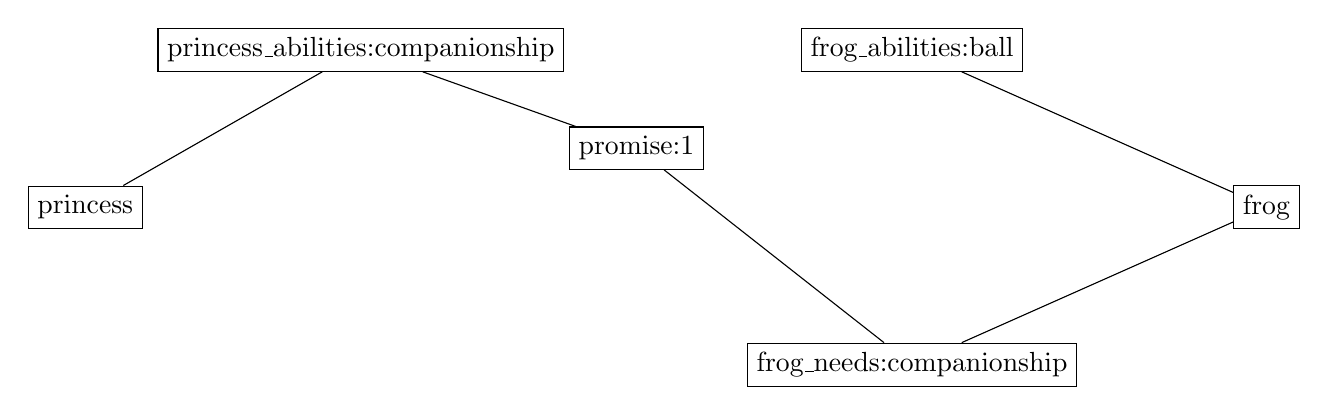
\begin{tikzpicture}
				\node[shape=rectangle,draw=black] (2p) at (0,0) {princess};
				\node[shape=rectangle,draw=black] (2pac) at (3.5,2) {princess\_abilities:companionship};
				\node[shape=rectangle,draw=black] (2pr1) at (7,0.75) {promise:1};
				\node[shape=rectangle,draw=black] (2fab) at (10.5,2) {frog\_abilities:ball};
				\node[shape=rectangle,draw=black] (2fnc) at (10.5,-2) {frog\_needs:companionship};
				\node[shape=rectangle,draw=black] (2f) at (15,0) {frog};

				\draw[-] (2p) -- (2pac);
				\draw[-] (2pac) -- (2pr1) -- (2fnc);
				\draw[-] (2fab) -- (2f);
				\draw[-] (2fnc) -- (2f);
			\end{tikzpicture}\\
			\textit{State 2}
		};
		\draw[-] (s1) -- (a1) -> (s2);
	\end{tikzpicture}
	\label{storyrep}
	\caption{Representation of a simple state-action-state transition.
	\textit{State 1}
	represents the part of "The Frog Prince" where the frog had promised to get
	the princess's golden ball from the bottom of a pond, in return for spending
	time with him (these promises are represented as relations between the
	rellevant abilities and needs of the princess and the frog). There is one
	action, where the frog gets the ball for the princess, which leads to the
	altered state in \textit{State 2} (The princess does not need the ball
	anymore, and the promise has been fulfilled, which is why both nodes have
	been removed from the graph).}
\end{figure}

\subsection{States}

States are represented as a graph of all currently active actors, their
abilities, and how these are connected with each other.
%TODO maak een plaatje van een state

\subsection{Actions}

Actions are represented as a short phrase (for example 
\texttt{"frog promise ball."}
or \texttt{"caliph transform into animal with magic\_powder"}).
These sentences are parsed with WordNet %TODO cite wordnet
to transform them into rule objects.

\subsection{Rules}

Rule objects are similar in form to action objects. These are extracted from 
the stories by seeing how states are affected by a certain action.
They can be represented as a tuple of $(a, \texttt{obj}, \texttt{subj}, \texttt{dat},
\texttt{prec}, \texttt{eff})$.

Here, the action is stored in a $a$ (for example "promise")

The dataset consisted of fairy tales, which often contain certain stock 
characters (the king, the princess, the witch, etc.)
This property is exploited by keeping track of a count of which agents
acted as objects, subjects, and (where applicable) datives in 
$\texttt{obj}, \texttt{subj}, \texttt{dat}$, respectively.
%In other genres this should probably replaced by certain properties the
%actors have instead of the actors themselves

$\texttt{prec}$ represents the preconditions of the action in terms of what 
relations certain actors should have with each other.
$\texttt{eff}$ represents the effects of the action in a similar fashion.
For example, if $a = \texttt{"kill"}$, $\texttt{prec}$ might be 
$ \{\texttt{hates}(\texttt{obj}, \texttt{subj})\} $ (you have to hate someone 
before you kill them), and $\texttt{eff}$ would be ${\texttt{delete}(\texttt{obj})}$
(if you are killed, you are removed from the next state).
Note that both $\texttt{prec}$ and $\texttt{eff}$ are sets of conditions.
An action can have multiple prerequisites and multiple effects on the story state.
